\section{Divide and Conquer}
\subsection{Multiplication}
\subsubsection{Problem Description}
For naive two n-digit multiplication with base 2, suppose n is 2's power.
\[
    xy=(a\times 2^{n/2}+b)(c\times 2^{n/2}+d)=ac\times 2^n+(ad+bc)\times 2^{n/2}+bd
    \]
    \[
        1234\times5678=(12\times100+34)\times(56\times100+78) 
    \]
    We only consider multiplication, ignoring multiplying by 100 (which can be done simply by shifting a few digits) or addition, which are linear compared to Multiplication.
    Eventually, we need $\log_2 n$ steps to divide into the base step (1-digit times 1-digit).With each step forward, we multiply to number of elements on the level by 4. 
    The multiplication is done on the end base, so in total we have $4^{\log_n2}=O(n^2)$ complexity.
\subsubsection{Karatsuba algorithm}
    Rather than calculating $ad,bc,ac,bd$ separately; we obtain $(ad+bc)=(a+b)\times(c+d)-ac-bd$.
    Therefore, instead of dividing it into 4 parts, we divide it into 3 groups, through 3 multiplication operations on $\frac{n}{2}$, we get $3^{\log_2n}=n^{\log_23}=n^{1.6}$
    Specially, if n is not 2's power, we add zero to max bits, which at most doubles the original length, $(2n)^1.6$.
    \begin{algorithm}
    \caption{Karatsuba algorithm}
    \textbf{Input:}Two n-digit numbers $x,y$. \\
    \textbf{Output:} their product\\
    $x_L,x_R=\text{leftmost} \lceil n/2\rceil ,text{rightmost} \lfloor n/2 \rfloor bits of x$ \\
    $y_L,y_R=\text{leftmost} \lceil n/2\rceil ,text{rightmost} \lfloor n/2 \rfloor bits of y$ \\
    P1=multiply($x_L,y_L$) \\
    P2=multiply($x_R,y_R$) \\
    P3=multiply($x_L+x_R,y_L+y_R$) \\
    return $P1\times 2^n+(P3-P1-P2)\times 2^{\frac{n}{2}}+P2$
    \end{algorithm}
    No adding Zero in real coding, since carrying occurs, (eg. 64-(32,(32+1)->64)).
    Time complexity is:
    \[
        T(n)=3T(\frac{n}{2})+O(n)= 3T(\frac{n}{2})+cn\\
        \]
    Due to carry, $T(\frac{n}{2})$ should be $T(\frac{n}{2}+1)=T(\frac{n}{2})+O(n)$.
\[  \begin{aligned}
    T(n)&=3\cdot(3T(\frac{n}{4})+\frac{cn}{2})+cn \\
    &=3^{\log_2 3}T(1)+cn(1+\frac{3}{2}+\frac{3^2}{2^2}+\cdots+\frac{3^{\log_2n}}{2^{\log_2n}})\\
    &=O(n^{\log_2 3})+O(n^{1+\log_2 1.5})\\
    &=O(n^{\log_2 3})=O(n^{1.6}) 
    \end{aligned}
    \]

    \begin{enumerate}
        \item \textbf{Toom-Cook}:$O(n^{1.465}$)\\
        Breaking into 3 parts $5\times\frac{n}{3}\times\frac{n}{3}$
        \item \textbf{Fast-Fourier Transform} 
        \item \textbf{Strassen's magical idea for Matrix Multiplication} \\
        Squeeze eight multiplications into seven with complex calculation, better than the naive case ($n$ for a row times a column, with $n^2$ numbers, in total $O(n^3)$. By normal divide and conquer, we divide one'n-size multi' into 8 $\frac{n}{2}$ multi, with total operations of $8^{\log_2n}=O(n^3)$)
    \end{enumerate}
    


\begin{remark}
    \textbf{Divide and Conquer} is a general algorithm design paradigm.
\begin{enumerate}
    \item \textbf{Divide} Divide the problem into small size subproblems.
    \item \textbf{Recursive} Solve small problems recursively
    \item \textbf{combine}  Combine the output of small size subproblems to get the answer for the original problem.
    \item \textbf{Basic solver} If the problem size is small enough, solve it directly.
\end{enumerate}
\end{remark}

\subsection{Sorting Problem}
% refer to fig:MergeSort:

A very familiar problem, which can be easily picked up by analyzing pipeline\ref{fig:MergeSort}.
\begin{figure}
    \centering
    \includegraphics[width=0.8\linewidth]{Notes/fig/MergeSort.png}
    \caption{Merge Sort Pipeline}
    \label{fig:MergeSort}
\end{figure}

\subsubsection{Time complexity}
For the 'merge' part, merging two arrays( length m and n) requires $O(m+n)$ time. For each level, we have $O(n)$ merging operations. There are $\log_2n$ levels, so the total time complexity is $O(n\log_2n)$

\begin{remark} Never use asymptomatic notations in an induction-based analysis!\\
An example of a wrong analysis is as follows:
\begin{prf} $T(i) = O(i)$ holds for $i=1,\ldots,n$ \\
\textbf{Base Step:} T1 =O(1) holds trivially.\\
\textbf{Inductive Step:} Suppose $T_i=O(i)$ holds for $i=1,\ldots,n-1$ \\
$T(n)=2T(\frac{n}{2})+O(n)=2O(\frac{n}{2})+O(n)=O(n)$ 
\end{prf}
There are two mistakes:

Firstly, the Inductive Step is meaningless, since $O(\cdot)$ takes in a function (with variable i). Given a specific value, $O(i=n-1)=O(1)$

Secondly, when the recursion happens numerous times, a constant can be a function of n. When we write $O(n)$, what we actually mean is $cn$.

Therefore, the correct proof should be:
\begin{prf} 
    $T(i) \leq ci$ holds for $i=1,\ldots,n$ \\
    \textbf{Base Step:} $T(1) \leq c$ holds trivially.\\
    \textbf{Inductive Step:} Suppose $T(i) \leq ci$ holds for $i=1,\ldots,n-1$ \\
    \[
    \begin{aligned}
    T(n)&=2T(\frac{n}{2})+O(n) \leq 2T(\frac{n}{2})+d\cdot n (\text{for some constant d})\\
    &\leq 2\cdot c\cdot \frac{n}{2}+d\cdot n (\text{ by induction hypothesis})\\
    &=(c+d)\cdot n
    \end{aligned}
    \]
    Induction fails as constant changes from $c$ to $c+d$.
\end{prf}
A correct proof should be:
\begin{prf}
    If $T(n) \leq 2T(\frac{n}{2})+c\cdot n$ for constant $c$, $T(n) \leq B \cdot n\log n$ for some constant \textbf{$B>c$}.
    \textbf{Base Step:} $T(2) \leq B\cdot 2\log 2$ holds trivially.\\
    \textbf{Inductive Step:} Suppose $T(i) \leq Bi\log i$ holds for $i=2,\ldots,n-1$ \\
    For $i=n$, we have\\
    \[
        T(n)\leq 2T(\frac{n}{2})+cn \leq 2\cdot B\cdot \frac{n}{2} \log \frac{n}{2}+cn=Bn \log n -Bn+cn < Bn \log n \]
\end{prf}
\end{remark}

\begin{remark}
    At least $\Omega(n\log n)$ comparisons are needed. //
    The time complexity is largely contributed by the running time of comparison.
    Total possible outputs is $3^{K(n)}$, n! numbers of permutations. Therefore, $3^{K(n)}\geq n!$, $K(n)\geq \log_3n! \geq \Omega(n\log n)$

\end{remark}

\subsection{Inversions}
\begin{defi}
    if $a_i>a_j$ when $i<j$, we call $(a_i,a_j)$ an inversion.
\end{defi}

The idea is that we divide the input into two subsets ( A:$x_1, x_2, \ldots , x_{m}$; B:$x_{m+1}, x_{m+2},\ldots, x_{m+n-1}$), and count the inversions of each subset and \textbf{across} subsets, which takes $O(mn)$ with each $a_i$ scanning the whole list B.

A magic trick is that we \textbf{mix merging and counting together}. We first count the inversions in A and B, then sort them separately.
If A,B are sorted, we change a 'comparison' complexity problem into a 'search' complexity problem.
In other words, we  insert the additional step of counting inversion in the mergesort, by following operations, with time complexity of O(nlogn).


\begin{algorithm}[H]
    \SetAlgoLined
    \KwIn{A list of n integers: S}
    \KwOut{Number of Inversions: count}
    count=0\\
    Divide the input into two subsets:
    A:$x_1, x_2, \ldots , x_{n/2}$; 
    B:$x_{n/2+1}, x_{n/2+2}, … , x_n$\\
    \If{$n==1$}{
        \Return{0}\\
    }
    \If{$n==2$}{

        \If{$x_1 < x_2$}{
            swap $x_1,x_2$\\
            \Return{1}
        }
        \Else{
            \Return{0}
        }
    }
    count+=countInversions(A)+countInversions(B)\\
    Maintain 2 pointers $i=1,j=n/2+1$ \\
    \While{$i < n/2$ and $j < n$}{
        \If{$x_i<x_j$}{
            $i+=1$
        }
        \Else{
            $j+=1$\\
            $count+=j-n/2$
        }
    }
    count+=(n/2-i)$\times $(j-n/2)\\
    \Return{count}
    \caption{countInversions}
\end{algorithm}
\begin{figure}
    \centering
    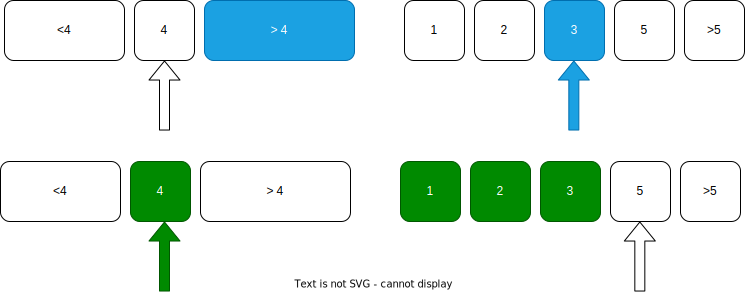
\includegraphics[width=0.8\linewidth]{Notes/fig/Inverse.png}
    \caption{Inversion}
    \label{fig:Inversion}
\end{figure}


\subsection{Master Theorem}
\begin{thm}
    If $T(n)=aT(\frac{n}{b})+O(n^d)$.\\
    a:Divide into a subproblems\\
    b:subproblem size n/b\\
    $O(n^d)$:combining time complexity\\
    \begin{equation}
        T(n)=
        \begin{cases}
            O(n^d) & \text{if } a<b^d\\
            O(n^{\log_b a}) & \text{if } a>b^d \\
            O(n^d \log n) & \text{if } a=b^d\\
        \end{cases}    
    \end{equation}

\end{thm}

\begin{prf}
The running time of solving size-1 problem is $O(a^{\log_bn})=O(n^{\log_ba})$.
The total running time for combining is $c\dot (n^d)+c\dot ((\frac{n}{b})^d)\dot a+\cdots a^k\dot c \dot (\frac{n}{b^k})^d+\cdots a^{\log_bn}\dot c$.
The size-1 problem complexity is eaten up by the last element of the combining complexity. 
Eventually, we have $c\dot n^d \dot (1+\frac{a}{b^d})+\cdots(\frac{a}{b^d})^k+\cdots(\frac{a}{b^d})^{\log_bn}$.
When $a<b^d$, intuitively the head is heavier(longer when imaging the operation of every layer as a line).
When $a>b^d$, intuitively the tail is heavier.
When $a=b^d$, $T(n)=O(n^d)\dot(1\times \log_bn)=O(n^d\log_bn)$.

\end{prf}

\begin{figure}
    \centering
    \includegraphics[width=0.8\linewidth]{Notes/fig/Master Theorem.png}
    \caption{Master Theorem}
    \label{fig:MasterTheorem}
\end{figure}




\subsection{Selection}
Input: A set S of n integers $x_1, x_2, \ldots , x_{n}$ and an integer k.\\
Output: The k-th smallest integer $x^*$ among $x_1, x_2, \ldots , x_{n}$.\\
naive case: Sorting and choosing the k-th element: O(nlogn)\\
alg 1: quick sort? have the first number to be the pivot.\\
alg 2: Divide $x_1,x_2,\ldots,x_n$ into three subsets, recursively pick out the subset $x^*$ is in.\\
\begin{algorithm}
    \caption{Select}
    Choose an \textbf{arbitrary} value $v$ among $x_1,x_2,\ldots,$\\
    Divide $x_1,x_2,\ldots,x_n$ into three subsets $L,M,R$\\
    \If{$k\leq |L|$}{
        return Select(L,k)
    }
    \ElseIf{$|L| < k \leq  |L|+|M|$}{
        return $v$
    }
    \ElseIf{$|L|+|M| < k$}{
        return Select(R,$k-|L|-|M|$)
    }
\end{algorithm}

\begin{prf}
\textbf{the scale of the problem shrinks:}

First, we show that the algorithm always terminates. If it does not terminate in the
current recursive iteration, it will either call Select(L,k) or Select(R, $k - L - |M|$).
It suffices to show that $|L|$ < n and $|R| $< n (so that the problem size is strictly
decreasing). This is guaranteed by $v \notin L$ and $v \notin R$ (v is in the set, so at least v is excluded).
\\
\textbf{the algrithm is correct inductively:}

Suppose the correct value is output for any array S of length n and any $k \in {1,2,\ldots,n}$. 
\textbf{Base Step:} n = k = 1, which is obviously true.\\
\textbf{Inductive Step:} Suppose the algorithm correctly outputs the k-th smallest value for
any array S with any length $l \in {1,2,\ldots,n-1}$ and any $k \in {1,2,\ldots,n}$.\\
Select(L,k) returns the k-th smallest value in L and Select(R, $k-|L|-|M|$) returns
the ($k-|L|-|M|$)-th smallest value in R by induction hypothesis.
For any input array of length n and any integer v in it, it is straightforward to check
that the k-th smallest value in L is the k-th smallest value in S if $L \geq k$, and the
remaining two cases are also correct.

\end{prf}

\subsubsection{Time Complexity}
For dividion,$\varTheta  (n)$ with each element compared to v. For recursion, $T(|L|)$ or $T(|R|)$ or $O(1)$.\\
For the worst case, consider ${1,2,...,n}$,where k=n. The algorithm is $O(n^2)$.

\begin{remark}
    Randomness in input and randomness in algorithm\\
    Commonly, we choose to analyze the mean time complexity of a random algorithm. 
    Because in real case, randomness of input is a strong condition(block-like features commonly).

    By estimation, for every layer, n comparisons. If we are lucky enough to have $\frac{1}{3}$ in the minimum separation, then $n\frac{2}{3}^n>1$, $k<\log_1.5n$.
    \begin{defi}
        $E[x]=\sum_{\omega \in \Omega}^{n} \Pr(\omega)\cdot X(\omega)  $
    \end{defi}
    \begin{thm}
        \textbf{Linearity of expectation}\\
        \[E| \sum_{i=1}^{n} X_i|=\sum_{i=1}^n E[X_i]\] 
        holds when $X_i,\ldots X_n$ are dependent.\\
    \end{thm}
    eg. For dices, $E[x]=\frac{1}{6}\cdot (1+2+\cdots+6)$. 
    When rowing two dices, by the Linearity of expectation, $E[x]=3.5+3.5=7$. If two dices output the same number magically, we still have $E(x)=(2+4+6+...+12)/6=7$.\\
\end{remark}

    For our case, since comparison takes up most of the running time, we calculalte the average times of comparison. Firstly, if $a_i,a_j$ are compared, one must be pivot and the other goes to the next layer of the division tree, which will only be compared once;
    When we consider the ordered sequence, $a_i, a_j$ are compared iff no element betweeen them are chosen as pivots, else they will be in different subsets, as is shown in \ref*{fig:randomComplexity}.
    \begin{figure}
        \centering
        \includegraphics[width=0.8\linewidth]{Notes/fig/ramdomComplexity.png}
        \caption{The white an are doesn't matter terms. We only consider the last step when $a_m , m \in [i,j]$ will be chosen as a pivot. There are (j-i+1) choices, and only 2 choices (namely, $a_i$ or $a_j$) can result in comparison between $a_i$ and $a_j$.}
        \label{fig:randomComplexity}
    \end{figure}
    
    \[
        E[X_{ij}]=\Pr(X_{ij}=1)\cdot 1 + \Pr(X_{ij}=0)\cdot 0=Pr(X_{ij}=1)=\frac{2}{j-i+1}\]

    \[
        i=1:\frac{2}{2}+\frac{2}{3}+\cdots+\frac{2}{n}=\sum_{i=1}^{n}\frac{2}{i}=2\cdot \sum_{i=1}^{n}\frac{1}{i}=2\cdot \log n\]
    \[
        i=2:\frac{2}{2}+\frac{2}{3}+\cdots+\frac{2}{n-1}\\
        \ldots
    \]
    To sum up, worst-case $O(n^2)$, expected average running time $\Theta(n\log n)$



\subsubsection{Median of the medians(1973)}

How to pick a \textbf{good pivot}? In other words, how to make sure $|L|$ and $|R|$ are approximately equal?

Partition $S$ into subsets with size 5. O(n)
Find the medians of each subset: $O(n/5)$ (since operations in a fixed-sized set is O(1)).\\
Find the median of the medians: $T(n/5)$.\\
Elements remaining: According to \ref{fig:medianofmedians}, there is $n-\frac{n}{5} \cdot \frac{1}{2}\cdot 3 = \frac{7n}{10}$ elements left.\\
\[
    T(n)=T(\frac{n}{5})+T(\frac{7n}{10})+O(n)\]
\begin{prf}$T(n)=O(n)$
    
Assume that $T(n) \leq cn$\\
$T(\frac{n}{5})<\frac{cn}{5}$,$T(\frac{7n}{10})<\frac{7cn}{10}$,
$T(n)=T(\frac{n}{5})+T(\frac{7n}{10})+O(n)<0.9cn+bn\leq cn$. which holds when we set c to be bigger then b.

\end{prf}

\begin{figure}
    \centering
    \includegraphics[width=0.8\linewidth]{Notes/fig/MofM.png}
    \caption{Median of the medians}
    \label{fig:medianofmedians}
\end{figure}

If the size of subset is i=2m+1, $m \in N$. To obtain the median of medians, we have $O(\frac{n}{2m+1})$. There are $n-\frac{n}{2m+1} \cdot \frac{1}{2}\cdot (m+1) = \frac{(3m+1)n}{2(2m+1)}$ elements left.
\[
    T(n)=T(\frac{n}{2m+1})+T(\frac{(3m+1)n}{2(2m+1)})+O(n)=T(\frac{(3m+3)n}{2(2m+1)})\]
However, in real case, the const is much bigger than 'quick sort' approach with a random pivot.


\subsection{Clostest Pair}
We can improve the naive algorithm by \textbf{sorting}. Imagine in 1-dim case, sorting ($O(n\log n)$) plus comparison between neighbouring points ($O(n)$) results in an $O(n \log n)$ algorithm.

Consider 2-dim case, apparently using only x sequence or y sequence cannot lead us to the right answer. Some tricks are implemented:
\begin{enumerate}
    \item \textbf{First sort by x, then by y}\\
    The only use of sorting by x is to divide the original dots into x-neighbouring subsets. After the division, any changes inside the subsets are allowed, so we merge the sort by y-axis step into the conquer step, which eliminates the $O(n\log n)$ sorting operation in each layer.
    \item \textbf{Bound the search plane}\\
    If we've found the minimum distance inside A and B separately, we only need to consider the distance between points across A and B. Additionally, $|x_i-x_{mid}|<dist$ ,which forms the $2-\delta strip$ shown in fig. 
    Similarly, during the conquer step, for each point $p_i$, we only consider $p_j$ that satisfies $|y_i-y_j|<dist$.
    By proposition \ref*{prp:fourPoints}, we magically found that only the distance between \textbf{four} neighbouring points are considered for each point (as is shown in fig \ref*{fig:closestPair})

\end{enumerate}
\begin{prp}
    At most 4 points can appear in a $\delta \times \delta$ square, so that the distance between any two points are no smaller than $\delta$.
    \label{prp:fourPoints}
\end{prp}
\begin{prf}
    Divide the square into four smaller squares, as in shown in fig \ref*{fig:fourPoints}. Since two points are at most $\frac{\delta}{\sqrt{2}}<\delta$ apart, at most one point can exist in each small square. So in total, at most four points appear in the square.
\end{prf}
\begin{figure}[htbp]
	\centering
	\begin{minipage}{0.3\linewidth}
		\centering
		\includegraphics[width=0.8\linewidth]{Notes/fig/fourPoints.png}
		\caption{At most 4 points appear in the square}
		\label{fig:fourPoints}%文中引用该图片代号
	\end{minipage}
	%\qquad
	\begin{minipage}{0.6\linewidth}
		\centering
		\includegraphics[width=0.8\linewidth]{Notes/fig/ClosestPair.png}
		\caption{Only four neighbouring points need to be considered for each point a}
		\label{fig:closestPair}%文中引用该图片代号
	\end{minipage}
\end{figure}

This brings out an $O(n\log n)$ alogorithm. The sorting by x-coordinate takes $O(n\log n)$, and the 'divide and conquer' step amounts to adding constant steps( since each point only has four neighbouring points to count) to MergeSort.

\begin{algorithm}
    \caption{FindClosestPair}
    \KwIn{A list of pairs P: $p_1=(a_1,b_1),\ldots p_i=(a_i,b_i),\ldots,p_n=(a_n,b_n)$}
    \KwOut{distance of closest two pairs in P: dist}
    
    \If{$|P|==1$}{return}
    Sort P by x-coordinate.\\
    Divide P into two equally sized subsets A,B, the point in the middle $p_{mid}=(a_{mid},b_{mid})$.\\
    dist=min(\textbf{FindClosestPair(A)},\textbf{FindClosestPair(B)})\\
    Merge A and B by y-cordinate to form C.\\
    \ForEach{$c_i=(a_i,b_i) $ in C}{
        \If{$|a_i-a_{mid}|<dist$}{ add $c_i$ to S}
    }

    \ForEach{$s_i=(a_i,b_i) $ in S}{
        j=i+1\\
        \While{$| b_i - b_{j}| <dist$}{
            dist=min(dist, $\| b_i - b_{i+1}\|$)\\
            j=j+1\\
        }
    }
    return dist
\end{algorithm}

\subsection{Fast Fourier Transform and Polynomial Multiplication}
We use array $(a_1,a_2,\ldots,a_{d-1})$ to describe $p(x)=\sum_{i=0}^{i=d-1} a_ix^i$
\[
    r(x)=\sum_{i=0}^{2d-2}c_ix^i, \text{where } c_i=\sum_{k=0}^{i}a_kb_{i-k}\]
By Karasuba Algorithm, we can have $O(n \log_{1.5} n)$ algorithm.
The key of interpolation is to use the minimum number of points to describe the original subject.
Any polynomial is a node in the n-dim space, with its coordinates $(a_1,a_2,\ldots,a_{d-1})$.
We need $2d-1$ interpolation points to fully store the answer polynomial by theorem .

\begin{thm}
    % matrix 
    \[
    \begin{bmatrix}
        y_0 \\ y_1 \\
        \vdots\\
        y_{d-1}
        
    \end{bmatrix}
    =
    \begin{bmatrix}
        1 & x_0 & x_0^2 & \cdots & x_0^{d-1} \\
        1 & x_1 & x_1^2 & \cdots & x_1^{d-1} \\
        \vdots & \vdots & \vdots & \ddots & \vdots \\
        1 & x_{d-1} & x_{d-1}^2 & \cdots & x_{d-1}^{d-1}
    \end{bmatrix}
    \cdot
    \begin{bmatrix}
        a_0 \\ a_1 \\
        \vdots\\
        a_{d-1}
        
    \end{bmatrix}
\]
Since the determinant of a Vandermonde matrix is $\Pi_{0\leq i < j \leq d-1}(x_j-x_i)$. Denote the middle matrix as A, A is an invertible matrix.

\end{thm}

\begin{figure}
    \centering
    \includegraphics[width=0.8\linewidth]{Notes/fig/FFT.png}
    \caption{FFT}
    \label{fig:FFT}
\end{figure}

interpolation step:
For counting $p(a_i)$, we need d addition for (2d-1) interpolations, which brings out $O(n^2)$.
However, we can try to compute $p(a_{i+1})$ from $a_i$ by carefully chosen interpolation points.
If we choose $a=\alpha$ and $a=-\alpha$, we can calculate $a_0+a_2\alpha^2+\ldots$ and $a_1+a_3^3+\ldots$ with d times, and reduce (2d) to obtain both $p(\alpha)$ and $p(-\alpha)$ with d times.

$T(D)=2T(\frac{D}{2})+O(n)$ is wrong, because the algorithm cannot be done recursively. In the second layer, $\alpha_0^2=-\alpha_2^2$ cannot be satisfied.
In the complex plane, however, for every element, there exists two roots.

multiplication of two complex numbers $r(a_i)-p(a_i)q(a_i)$\\
recovery: 
% big matrix
How to find $A^{-1}$ and calculate matrix multiplication?
\[
    \left(
        \begin{matrix}
            
        \end{matrix}
        \right) 
\]

% inner product of 2 complex numbers: 
% a,b=\sum_{i=1}^{n} \overline{a_i}\cdot b_i 
% orthogonal,orthonormal(unitary)
If columns are orthonormal, so are the rows.
$AA^{*}=E$,$A^{-1}=A^*$. Intuitively, the inverse of a orthonormal matrix can be obtainly easily.\\
\begin{prp}
    $\frac{1}{\sqrt{D}}A(w)$ is orthonormal for $w=e^{\frac{2\pi i}{D}}$
    
\end{prp}